
% thesis.tex (also saved as simple.tex) -- a simple thesis document
% for demonstrating dalthesis.cls class file, or to use as a starting
% document for writing a thesis.
% If you are not familiar with TeX and LaTeX, the first thing that you
% can learn that line comments start with the percent sign (%), so
% these lines are ignored by the system.  Feel free to change them or
% delete them.
\documentclass[12pt]{report}
\newcommand{\mychapter}[2]{
    \setcounter{chapter}{#1}
    \setcounter{section}{0}
    \chapter*{#2}
    \addcontentsline{toc}{chapter}{#2}
    }
\usepackage[utf8]{inputenc}
\usepackage{graphicx}
\usepackage{gensymb}
\usepackage{comment}
\usepackage{amsmath}
\usepackage{caption}
\usepackage{subcaption}
\usepackage{pdfpages}
\usepackage[toc,page]{appendix}
\usepackage{afterpage}

\newcommand\blankpage{%
    \null
    \thispagestyle{empty}%
    \addtocounter{page}{0}%
    \newpage}
\usepackage{hyperref}

\pagenumbering{roman}

\begin{document}


\begin{figure}
 \centering 
 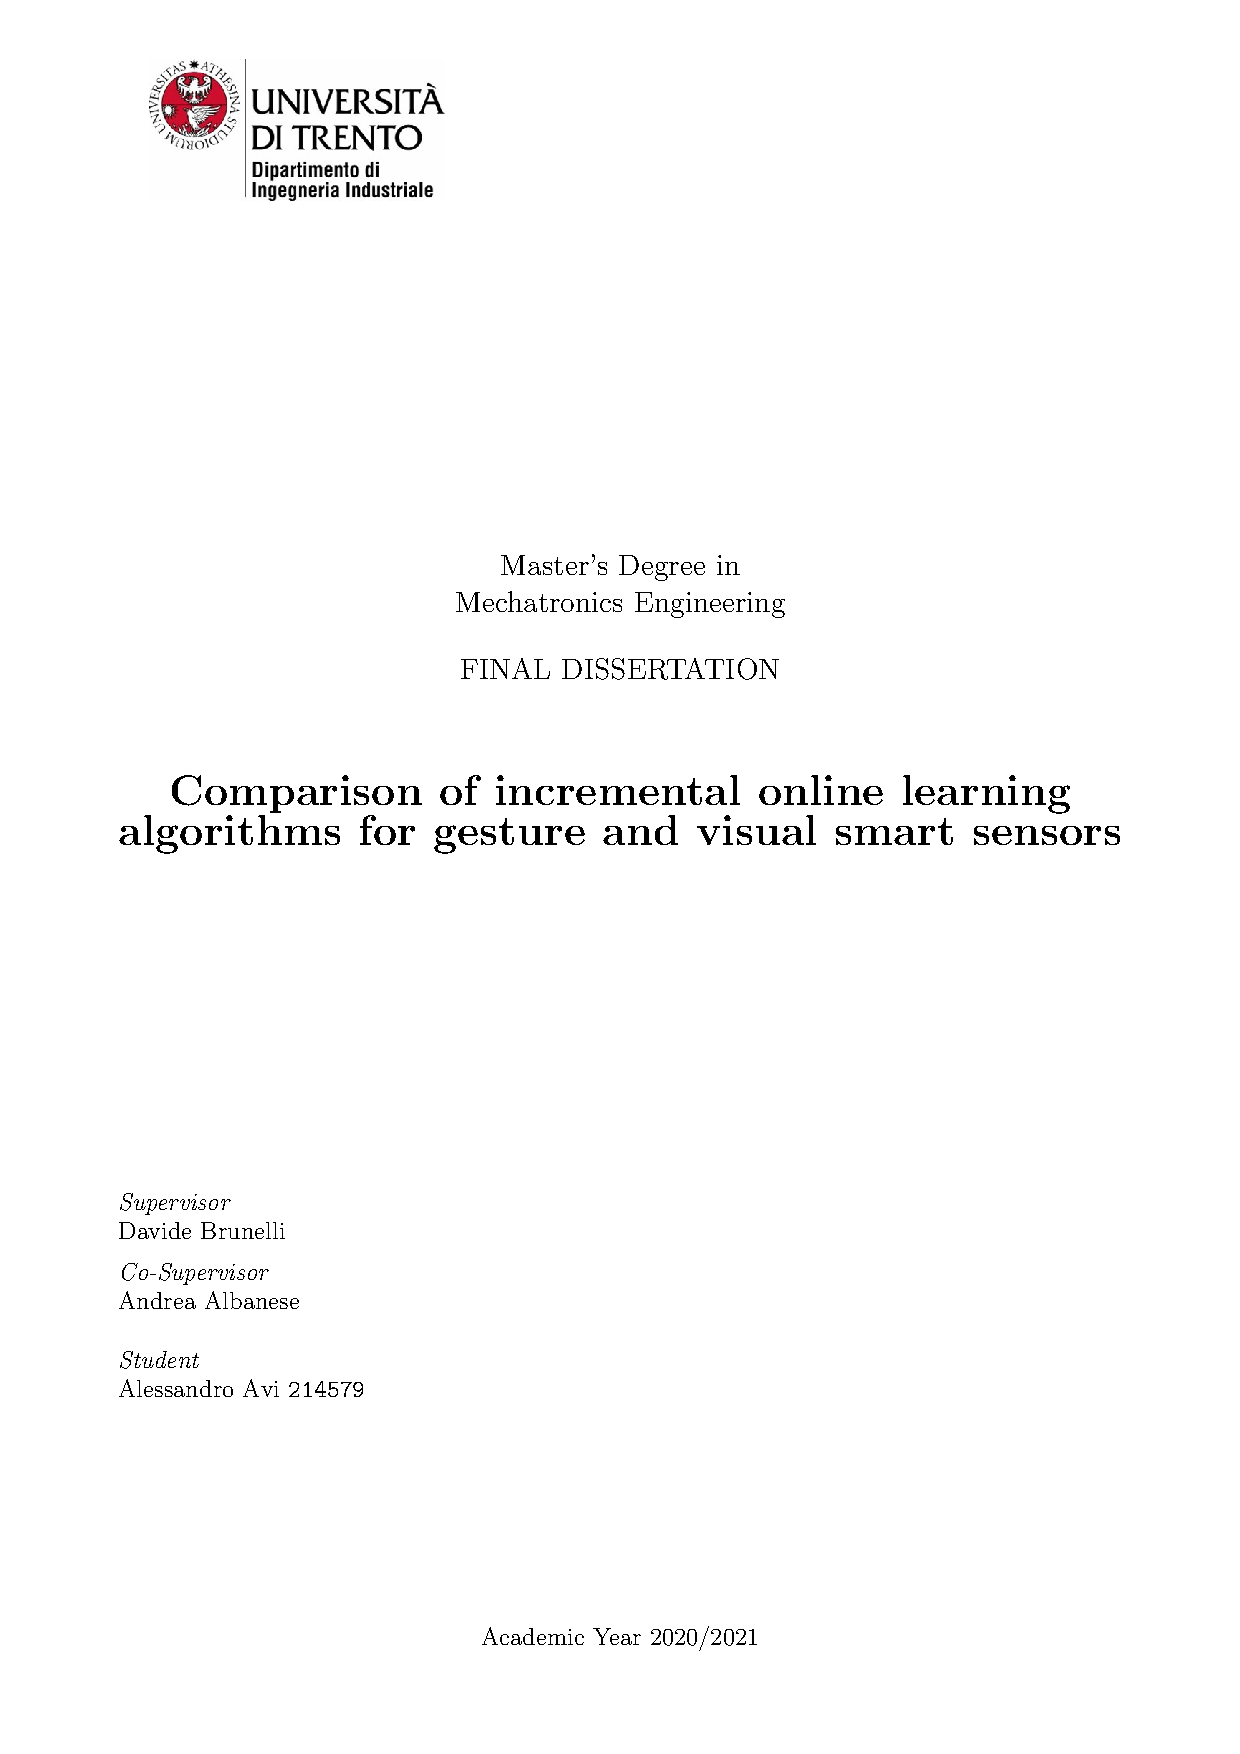
\includepdf[pages=-]{Figures/frontespizio.pdf}
\end{figure}

\afterpage{\blankpage}

\chapter*{}
\vspace*{\fill}
\textit{"Ciao."} 
\begin{flushright}
Mario
\end{flushright}
\vspace*{\fill}

\afterpage{\blankpage}





%\afterpage{\blankpage}
\tableofcontents
%\afterpage{\blankpage}
\listoffigures
\listoftables
\afterpage{\blankpage}



%\mainmatter

\mychapter{0}{Introduction}
\pagenumbering{arabic}

The application of machine learning (ML) on small devices, in a word TinyML, is becoming more and more popular as technologies advances. The usage of this type of technology on micro controllers (MCU) is proving to be more indispensable and helpful in several fields like the industrial applications, agricultural automation, autonomous driving, human-machine interaction. One of the main fields in which TinyML shines and is well suited is the world of Internet of Things (IoT). Here machine learning applied on small devices finds its sweet spot since it can be exploited to revolutionize the basics of IoT networks. The ability of embedded systems to perform high level and smart data elaboration makes it possible for the IoT pipeline to change from cloud computing to edge computing. This transformation comes with great benefits and additional challenges. 
First of all the traffic on IoT networks is drastically reduced. In fact by performing inferences and predictions directly on the edge the raw data gets compressed into smaller sequences that are enriched of information, reducing the quantity of data moving int the IoT networks. This allows to reduce the energy consumption dedicated to the entire system. In fact by redirecting the energy flow from data transmission to ML computation it's possible to decrease the consumption by and order of magnitude \cite{} SERVE UNA REFERENCE. 
Not only edge computing lowers the traffic but also it reduces the computational weight given to the central point of the entire network, the cloud. This results in reduced times of computation and communication between edge and cloud, which if combined with the ability of the MCU to perform autonomous decision, reduces the latency of real time applications improving the overall experience. 
Another benefit is the improved privacy of the network which is a direct consequence of the reduction of data transmitted. Of course by having less data transmitted alsothe possibility to have unwanted interceptions is reduced. At last the usage of ML on small devices allows for better customization of the device itself, which can make the devices better suited for the job. 
Of course the application of such a technology comes with a cost, in this case increased complexity and higher amount of vulnerabilities. It's in fact necessary to set up robust systems that are able to ensure the security of the system (due to the high number of vulnerable nodes) and perform at their best, no matter the limitation of the device. It's known that the main downsides of embedded systems and small MCUs are their limited hardware, mainly small memories and batteries. Still these devices are required to perform at their best even with limited computational power and limited power consumption.\\
Another relevant challenge for the application of ML in the world of IoT comes directly from the environment in which these are deployed. Depending on the specific application it's usually the case that the context in which an IoT device lives is not characterized by static behaviour. Meaning that the phenomenon to be monitored is able to change or evolve over time and so does the data recorded. This can make difficult the usage of the ML models because they lack the ability to adapt to the changing scenarios. In fact typical TinyML applications aim at training the models on powerful devices and later deploy them on the MCU, where only the inference is performed. It's clear how these devices are vulnerable to the context change before mentioned. In today's research three different types of scenarios can be defined: New Instances (NI), when new patterns of already known classes are detected; New Classes (NC), when new families of data are found that are not recognized by the system ; New Instances and Classes (NIC), when the data is composed of both new patterns and new classes.
By training ML models for a specific context and later deployng them in the real world is to be expected a drop in prediction accuracy which would make the application itself non reliable. It's then clear how an application of simple ML on such problems is not the best solution. In order to contrast the issue it's necessary to implement what is called Continual Learning (CL). A machine learning approach that allows ML models to be continually kept up to date
This type of machine learning method uses a real time training based on the data incoming, thus allowing the model itself to change and adapt its weights to better contrast the context drift. An additional feature that can be easily added to CL is the recognition of new and never seen classes, that allows the model to also extend its structure in order to better perform inference on the data and be able to recognize new classes. \\
The implementation of CL in industrial applications is not a new topic in the research world, but its implementation on tiny devices is just starting to become more and more popular. The most common applications see CL in industrial scenarios, mainly for monitoring purposes on heavy machines.
The main contributions of this study concern the application of CL in two interesting application. The objective here is to understand if CL is a feasible solution for TinyML and if its usage is actually effective for the generation of autonomous and self adapting models. In this study several state of the art continual learning algorithms are implemented and tested in two experiments, both concerning the application of ML classification on different types of data. The first application regards the analysis of accelerometer data. In this experiment the user holds the accelerometer sensor in its hand and records a time series of accelerations while drawing letters in the air. The idea is to be able to apply ML in order to classify the input data are recognize the letters written. The model created is initially trained for the recognition of the pattern from the vowels. Later CL is applied to the experiment and the model is exposed to new data representing three new consonants. The aim of the experiment is to let the ML model learn the new patterns by performing a real time training. Even if the experiment proposed is closer to an academic study than a real application it's considered to be a clear example of how a CL model could behave in a similar scenario. A popular application of CL in the research is in fact the monitoring of vibration patterns of heavy industrial machinery. The second application sees the experimentation of CL on a CNN model applied on an OpenMV camera for the recognition of the digits from the MNIST dataset. The idea this time is to initially train the model to recognize only the digits from 0 to 5 and later use the CL framework developed for applying a real time training on the remaining digits. This second experiment could be closer to an application, once again in the industry field, where a camera is used for visual control of defects on products in a production pipeline.  \\
The work done for this study is a good example for showing the capabilities of these tiny devices. It proves that machine learning applied on MCUs is a technology that has huge potential and deserves more attention. It could lead to smarter, more efficient, better performing systems in the fields of IOT and applications in the industrial and agricultural world. 

%accennare catastrophic forgetting



\chapter{Related Works}


\section{Machine learning in general}


\section{Machine Learning on MCU}
% applicazione ml su mcu, risorse limitate, molto importante power comsumption, design del mcu, paralre di possibili applicazioni, paraldre del fatto che si fa solo inference
% parlare del rpuning, binarization, compression del meodello, state of teh art compression MCUNET


TinyML is a fast growing research area that aims at applying ML on limited devices like micro controllers. This technology has found a rapid grow in the last years especially thanks to the potential demonstrated by useful applications. The main fields in which TinyML can be applied are human-computer interactions, industrial applications, ... Fare esempi di paper generici su TinyML

The main challenge of TinyML is for sure the successful application of ML on such resource constrained systems. These are in fact designed to be deployed in difficult to reach places and for running for very long times. This implies that the devices should be battery powere or equipped with energy havresting hardware and their power consumption should be limited and optimized. Other limitations concern the limited computational power, which is directly connected to the CPU frequency and the battery management and the available memory. The latter is a very important topic for TinyML. It's in fact known that the application of ML on any type of device requires the usage of great amounts of memory, it's then a big challenge to be aple to deploy these systems with very limited memories.\\
The application of ML on MCUs, mobile devices or in general on the edge of IoT systems it's a great advantage that can bring to some improvmenets. The key advantages are:
\begin{itemize}
\item privacy: by having the data directly processed on the node there is no change of violating the privacy policies since the possibility of interception is totally nulled
\item latency: by elaborating data directly on the edge the work load of processing that should be performed by the cloud is limited and so is the transmission of the data itself. This brings to limited time delays and allows the device to perform decisions in real time, improving the performances of real time applications.
\item energy efficiency: the transmission of huge quantities of data from the edge to the cloud takes a big portion of the energy consumption of an IoT system. Even if the application of NN is energy intensive it is an order of magnitude less, thus an improvement.
\end{itemize}


\section{Continual-on line learning}
% spiegare cosa è ctastrophic forgetting, come mai serve, cosa va a risolvere, quali sono i problemi che iontroduce, 
% parlare di cinme CL è trattato nella research, paralkre dlle tipologie di algoritmi, supervised training, frameworks gia sviluppatim metodi di valutazione?

Until recent times the application of ML on MCUs has always been focused on the creation of intelligent small system that maintain good performance with reasonable consumption, limited time of inference and long lifetimes. A major negative aspect of the TinyML solutions is their focus on the inference of streams of data. Which almost always requires the usage of powerful machines for the training of NN models that are later deployed on the MCU. This results in the creation of a static network which is not able to adapt to the data and adjust to different scenarios. The solution to this problem is the creation of a Continual Learning system. \\
CL systems are a variation of the tipical pipeline of ML. The main focus of CL systems is to be able to continuously update the model in order to adapt its structure and parameters to overcome context drift, be able to recognize appearance of new patterns and to avoid catastrophic forgetting. The latter is a problem that is directly introduced by the nature of the paradigm itself. By having a model that is continuously updated with a feedback loop that is directly dependent on the current erross i'ts clear how it's immediate to update the model in such a way that the old tasks are forgetten for the sake of learning the new ones. This could be seen also as a over fitting of the model on the new tasks and if oc course to be avoided. Different algorithms have different ways for contrasting this phenomenon. \\
In todays literature several CL algoprithms and strategies have been already proposed. A well organized summary is proposed in \cite{lesort2020continual}, where the most relevant methods are briefly classified in 4 categories, originally proposed by \cite{maltoni2019continuous}.
\begin{itemize}
\item Architectural: these algorithms are based on the usage of particular types of structures and architectures. Some common methods are weight-freezing, layer activation or dual-memories-models that try to imitate logn term memory and short term memory.
\item Regularization: this group contains all those approaches that base their ability to retain past memories on the application of particular loss functions. In these loss functions usually a term is added with the aim of performing a feedback that considers both the old knowledge and tries to learn the new data.
\item Rehearsal strategies: in these strategies past informations are periodically revisited by the model. This is done for strengthening the old knowledge and connections. Notice that this methods is not well suited for application on MCUs mainly because of the restricted memories. 
\item Generative Replay: this methods implement similar strategies of the rehearsal. This time the data that is repeated in the models is not actually old data saved in the memory but it's actually data artificially generate by the model itself. 
\end{itemize} 

The type of strategies that better suits an application on MCU are for sure the regularization methods and the architectural methods. Both these groups require little to no extra computation with respect to a simple ML application, thus their strength is intrinsic in the update rules adopted. Some of the most important methods from the state of the art are, LWF, PNN, CWR, EWC, SI. 









\chapter{Hardware} 








\chapter{Machine Learning}





\chapter{Experimental set up}

In this chapter the practical aspects of the experiments are explained. Initially the study has been developed entirely on the laptop with the aim of understanding the capabilities of CL and if such an application could be applied on micro controllers. The part developed on the laptops has been written entirely in Python. Python is a simple and flexible language that is widely used for machine learning applications. The presence of powerful libraries and tools, such as Tensorflow and Keras, make the development of ML models and the creation of applications very fast and easy to understand. \\

\section{Dataset generation}

In order to be able to create ML models it's necessary to have large quantities of data for the trainings. In this study the two application explored see the usage of accelerometer data and images from the MNIST dataset. The MNIST digits dataset is a publicly available dataset of hand written digits. These images are widely used in the research and academic world mainly because of its high number of samples (xxx samples), ease of use, high quality data and free availability. For the purpose of this study application the dataset is manipulated before use. Since the goal of the model is to be able to correctly recognize the digits from 0 to 6 it's necessary to separate the dataset in $low\_digits$ and $high\_digits$. Once this is done two dataset are obtained. The $low\_digits$ dataset contains xxx samples, while the $high\_digits$ dataset contain xxx samples. In order to be able to use the dataset for the training of the frozen model it's necessary to divide the dataset in train, validate and test portions. In this case it has been decided to use the common rule 70-10-20. \\
On the other hand for the accelerometer application it was necessary to create a dataset from zero. To my knowledge there are no publicly available datasets containing accelerometer data of letters written in the air. The collection of the dataset has been done with a MCU equipped with an accelerometer sensor. The MCU used is the same from the training, a Nucelo STM32 F401-RE, while the accelerometer sensor is contained in the STM shield IKS01A2. The dataset is composed of 8 different letters, which are A, E, I, O, U, B, R, M. The vowels are the classes that are learned by the original model, while the 3 consonants are the letters that are learned by the CL system. During the collection of the dataset the MCU should be connected to a laptop which behaves as power sourec and memory device for the data. The Nucleo contains a small script that allows the user to record the stream of data from the sensor in real time. Once the blue button is pressed the MCU starts to collect accelerometer data from the sensor with a frequency of 100 Hz and for a period of 2 second. While the data is recorder from the MCU it's also sent via UART protocol to the laptop. Here a software for serial communication should be used, in my case MobaXTerm was the software of choice. Once the data collection is done it's possible to save the entire data stream in a txt file. One data sample is composed of several information which are the number of sample taken in the current session, the label of the letter written in the air and the accelerometer data from the three axis of the accelerometer. The accelerometer data is recorded from the 3 axis, this means that a sample is composed of a matrix of shape $3 \times 200$, where 200 is the time series cause by a frequency of 100 Hz that lasts 2 seconds. The final dataset is composed of xxx samples, where the vowels have circa xxx samples, while the consonants have circa xxx each. The motion used for the recording of the letters followed always the same approximate path. In order to have a dataset as close as possible to a NIC scenario it has been decided to record the letters with the same approximate motion but accentuated characteristics. Some examples are the different velocities at which the sensors moved, more accentuated angles, more or less accentuated curves for the letters O and U ecc. In Figure[\ref{fig:letters_motion}] are shown the motions folloed for each letter.




\begin{figure}[h!]
    \centering
    
\includegraphics[width=100mm]{Figures/Chapter4/letters_motion.jpg} 
    \caption{Motion of the accleerometer}
    \label{fig:letters_motion}    
\end{figure}

\section{Implementation of the algorithms}

\section{Trainin of the models}

\section{Deployment on the MCU}









\chapter{Experimental results} 






\chapter{Conclusion}





\bibliographystyle{IEEEtran}
\bibliography{thesis}

%\clearpage
%\pagenumbering{arabic}% resets page counter to 1
%\renewcommand*{\thepage}{A\arabic{page}}

%\renewcommand\appendixname{Appendix}
%\renewcommand\appendixpagename{Appendix}
%\renewcommand\appendixtocname{Appendix}

%\begin{appendices}



%\end{appendices}

\end{document}
